\documentclass[sigconf,nonacm]{acmart}
\usepackage{booktabs}
\usepackage[ruled,linesnumbered,vlined]{algorithm2e}
\usepackage{xspace}
\usepackage{tikz}
\usetikzlibrary{arrows.meta,positioning}
\usepackage{pifont}
\usepackage[capitalise,noabbrev]{cleveref}
% a little extra stretch keeps two-column lines inside the margin
\setlength{\emergencystretch}{1em}
% columns end where the text ends; no stretched gaps around a top float
\raggedbottom

\definecolor{sysc}{HTML}{0072B2}   % TGSA and its structures (blue)
\definecolor{wins}{HTML}{D55E00}   % insert path (vermillion)
\definecolor{qnbr}{HTML}{009E73}   % queries Q1--Q4 (green)
\definecolor{qwin}{HTML}{009E73}   % same green; kept as a name for the drawings

\newcommand{\sys}{TGSA\xspace}
\newcommand{\tmap}{\texttt{tmap}\xspace}
\newcommand{\challenge}[1]{\textbf{(C#1)}}
\newtheorem{example}{Example}

% ---- headline numbers, defined once so that the abstract, the
% introduction, the evaluation and the conclusion cannot disagree.
% Source: results/e33_matrix/e33.csv (aligned matrix), results/e18_recovery.
\newcommand{\nLanlEvents}{1.05B}
\newcommand{\nSmallEvents}{7.8M}
\newcommand{\nIngestMin}{33.3}      % slowest TGSA ingest rate, M events/s (THEIA)
\newcommand{\nIngestMax}{72.5}      % fastest TGSA ingest rate, M events/s (LANL)
\newcommand{\nIngestGapLo}{1.6}     % advantage over GraphOne on the three corpora where TGSA leads
\newcommand{\nIngestGapHi}{1.9}
\newcommand{\nIngestRestLo}{4}      % advantage over every other system
\newcommand{\nIngestRestHi}{2{,}400}
\newcommand{\nRecoverSec}{29.6}
\newcommand{\nStructuralGap}{2.0}   % median TGSA/CSR storage share, BFS/PR/LP on four corpora
\newcommand{\nSingleCallLo}{60}   % one-batch ingest, slowest corpus (wiki-talk), median of three
\newcommand{\nSingleCallHi}{86}   % one-batch ingest, fastest corpus (CADETS)
\newcommand{\nDurWriteLo}{50}    % write-only log cost, percent of peak (wiki-talk)
\newcommand{\nDurWriteHi}{66}    % (LANL)
\newcommand{\nDurDiskLo}{2.9}   % async 4 MB commit, wiki-talk
\newcommand{\nDurDiskHi}{5.4}   % async 4 MB commit, CADETS

\begin{document}

\title{TGSA: A Time-Keyed Storage Engine for Temporal Event Analytics}

\author{Anonymous submission}
\affiliation{\institution{}\city{}\country{}}

\begin{abstract}
Graph storage has spent two decades optimizing for structure: layouts, indexes, and update paths are organized around vertex identity, while timestamps are stored as payload attributes. Many emerging workloads, however, are organized around time. Network flow analysis, system provenance, execution traces, and interaction logs build graphs from immutable timestamped events that arrive continuously, are queried by window, recency, and causal order, and are retained under time-based policies. We call this workload \emph{temporal event analytics}. A structure-keyed layout makes each of these operations recover temporal order indirectly: a window query becomes a scan with a filter, retention becomes a scattered delete, and a separate time index must be maintained on every write and reconstructed after a crash. This paper presents \sys, a storage engine that keys temporal event graphs on time itself. First, \sys introduces the \emph{temporal address space}: each timestamp maps to a virtual address by a subtraction and a shift, demand paging absorbs temporal sparsity, and no index is built, maintained, or recovered. Second, ingestion, the appending of arriving events, claims runs of same-window arrivals with single atomic operations under a per-slot publication protocol, so queries stay correct \emph{during} lock-free multi-writer ingestion and correctness does not depend on arrival order. Third, because a time prefix is an address prefix and engine state is a pure function of the appended multiset, retention is a page release and recovery is a replay. On four event datasets from \nSmallEvents{} to \nLanlEvents{} events, \sys ingests \nIngestGapLo{} to \nIngestGapHi{} times faster than the fastest competing store on three datasets and matches it on the fourth; relative to every other system, it is \nIngestRestLo{} to \nIngestRestHi{} times faster. \sys also answers window scans and time-respecting traversals faster than every system on every dataset, by 3 to 15{,}000 times, and wins 27 of 32 windowed-neighbor and as-of comparisons. The five losses occur on hub-dominated queries, where GraphOne's archived adjacency is 1.5 to 4.7 times faster. On whole-graph structural algorithms, \sys pays a bounded overhead of about \nStructuralGap{} times relative to a static layout that cannot ingest.
\end{abstract}

\maketitle

% =====================================================================
\section{Introduction}\label{sec:intro}
For two decades, graph data management has focused primarily on
structure. Systems research has optimized neighborhood
layout~\cite{dhulipala2019aspen, deleo2021teseo, fuchs2023sortledton},
adjacency compression~\cite{wheatman2021ppcsr, pandey2021terrace}, and
structural update paths~\cite{kumar2019graphone, zhu2020livegraph,
shen2026dcsr}, and has evaluated them largely with structural queries
and whole-graph analytics~\cite{malewicz2010pregel, shun2013ligra, kyrola2012graphchi, zhu2016gemini}.
For an important class of modern workloads, however, time rather than
structure determines the critical path. Network flow
analysis~\cite{lakhina2004anomalies, cranor2003gigascope, gupta2018sonata}, system
provenance~\cite{king2003backtracker, pasquier2017camflow, hossain2017sleuth, han2020unicorn}, execution
traces~\cite{hassan2020omegalog, milajerdi2019holmes}, and interaction
logs~\cite{leskovec2014snap, paranjape2017motifs} build graphs from \emph{events}: a flow
record, a system call touching a file, a host authenticating to
another~\cite{lanl2015data}. Each event records when it happened, is immutable once appended, and
arrives as part of a continuing stream. The common questions are
therefore temporal: which events fall inside a window, which earlier
events could have reached this host in time
order~\cite{kempe2002temporal, wu2014temporalpaths, holme2012temporal}, and which events
have crossed the retention horizon. We call this
workload \emph{temporal event analytics}; its critical path runs
through the timestamp.

\begin{figure}[t]
  \centering
  \includegraphics[width=0.95\linewidth]{figures/fig_motivation.pdf}
  \caption{\small The CADETS intrusion as a temporal event graph
  (Example~\ref{ex:cadets}).}
  \label{fig:motivation}
\end{figure}

\begin{example}[The CADETS intrusion]\label{ex:cadets}
CADETS is a whole-system provenance trace from the DARPA Transparent
Computing program~\cite{darpa2020tc}: 22.5M information-flow events
from one FreeBSD host over eleven days, with a documented red-team
intrusion inside. The intrusion is a chain of events in time order
(\cref{fig:motivation}): an implant is dropped, a privilege is
escalated, command-and-control traffic starts, a process is injected.
When the alert fires, the analyst asks two questions: looking
backward, which earlier events could have caused it; and looking
forward, what the compromised process touched afterwards. At the
same time, new trace events continue to arrive while the retention
policy removes the oldest ones. Ingestion, investigation, and
retention therefore all operate along the same time axis.
\end{example}

Existing storage engines serve this workload with layouts built for the
structural era, and each layout makes it pay. Dynamic graph
stores~\cite{kumar2019graphone, zhu2020livegraph, dhulipala2019aspen,
fuchs2023sortledton, deleo2021teseo, ediger2012stinger} key storage on
the source vertex and treat the timestamp as payload: a window query
becomes a scan of every neighborhood with a per-edge filter, and
retention must find expired edges wherever vertex order scattered them.
Log-structured and columnar engines~\cite{oneil1996lsm, luo2020lsmsurvey, dong2021rocksdb,
raasveldt2019duckdb} order records by time, which recovers the window
scan, but a traversal then pays a join per hop, and a log-structured
merge (LSM) store rewrites every record at each merge. Versioned
temporal graph databases~\cite{li2026tva, hou2024aeong,
theodorakis2024aion, huang2016tgraph} retrieve the valid \emph{version} of an updated
entity; their delta encoding and version-chain locality presume few
versions per entity, and an event stream, in which every repeated
contact is a new event, violates that premise by construction. A
statically time-sorted compressed sparse row (CSR) layout answers
temporal queries nearly optimally but cannot ingest: its only update is
a full rebuild.

Across these designs, locating data by time still requires an
indirection: an explicit tree, a maintained sort order, or a scan that
filters by timestamp. \sys removes this indirection. Because a 64-bit
virtual address space is far larger than the time span of practical
traces, a timestamp need not be looked up in an index; it can
\emph{determine the address directly}.
We present \sys, a storage engine built on that observation. Its \emph{temporal
address space} (\S\ref{sec:tmap}) maps a timestamp to an address with
one subtraction and one shift, and demand paging absorbs temporal
sparsity, so locating events by time costs no data structure
(Challenge~1: no index). Ingestion is lock-free. Because consecutive arrivals usually share a
time window, a writer claims a run with one atomic operation
(\emph{run claiming}) and publishes each event with one release store.
Queries therefore remain correct during multi-writer ingestion, and
correctness does not depend on arrival order (Challenge~2: correct reads without sorting on
the write path). A time prefix is an address prefix, so retention is a
page release; engine state is a pure function of the appended multiset,
so recovery is replaying a checksummed log through the ordinary insert
path (Challenge~3: bounded resources under a stream that does not end).
\emph{Compaction}, the pass that sorts each vertex's references by
time, is optional and off the ingest path: it changes query cost, never
answers. What the layout gives up is organization by vertex, and
\S\ref{sec:eval} measures that price.

This paper makes four contributions. First, it presents \sys, a
storage engine that keys temporal event graphs directly by time, with
formal properties for addressing, space, granularity, concurrency, and
recovery. Second, it defines the temporal address space as a reusable
contract whose guarantees apply to any client that appends data into
its slots. Third, it introduces run claiming and a per-slot publication
protocol for lock-free ingestion, and proves that readers never observe
partial state during concurrent multi-writer updates. Fourth, it
evaluates \sys against seven systems on four datasets ranging from
\nSmallEvents{} to \nLanlEvents{} events and on the same four query
types; every answer is verified before timing, recovery is tested by
fault injection, and the major design choices are measured in
isolation.

% =====================================================================
\section{Background}\label{sec:background}
\subsection{Temporal Event Graph Model and Query Set}\label{sec:model}
A temporal event graph is $\mathcal{G}=(V, E)$ where $E$ is a
\emph{multiset} of events $e=(src,dst,t,w)$ with $src,dst \in V$, a
timestamp $t$, and a weight $w$. Events are immutable: once appended,
an event is never updated, and deletion exists only as retention
policy. The supported operations are exactly the lifecycle of a stream:
\textbf{append}$(e)$ adds an event; \textbf{evict\_before}$(t)$
discards every event with timestamp below $t$;
\textbf{replay}$(L)$ re-appends a logged prefix after a failure. A
query is a predicate over the multiset,
\begin{equation}
Q \;=\; \{\, e \in E \mid P(e) \wedge e.t \in [t_1, t_2] \,\},
\label{eq:query}
\end{equation}
optionally closed under time-respecting reachability: a path
$v_0 \rightarrow^{e_1} \cdots \rightarrow^{e_k} v_k$ is
time-respecting when $t(e_1) \le \dots \le t(e_k)$. Temporal event
analytics issues four kinds of queries; \cref{tab:queries} names them
once and the rest of the paper uses the names. Q1 and Q2 are
\cref{eq:query} over time alone and over one vertex; Q3 is its closure
under time-respecting paths, the two questions of \cref{ex:cadets}; Q4
is the neighborhood of a vertex as it stood at time $t$, the operation
versioned graph stores are built around. Whole-graph algorithms that
ignore timestamps are not the target workload; \S\ref{sec:eval-structural}
prices them anyway.

\begin{table}[t]
\centering\footnotesize
\setlength{\tabcolsep}{4pt}
\caption{\small The query set.}
\label{tab:queries}
\begin{tabular}{@{}llp{40mm}@{}}
\toprule
Query & Input & Output \\
\midrule
Q1 window scan & $[t_1,t_2]$ & every event with $t_1 \le t \le t_2$ \\
Q2 windowed neighbors & $v, [t_1,t_2]$ & every out-event of $v$ with $t_1 \le t \le t_2$ \\
Q3 time-respecting traversal & $v, [t_1,t_2]$ & every vertex reachable from $v$ along a time-respecting path inside $[t_1,t_2]$, with the earliest time it is reached \\
Q4 as-of neighbors & $v, t$ & for each distinct neighbor $u$ of $v$, the latest event $v \to u$ with timestamp at most $t$ \\
\bottomrule
\end{tabular}
\end{table}

This model is intentionally narrower than a general property graph: it
excludes vertex properties, in-place updates, and multi-event
transactions. \S\ref{sec:tmap} states what the restriction buys and
\S\ref{sec:eval} what it costs.

\emph{Relation to Versioned Temporal Graphs.} Systems such as
TVA~\cite{li2026tva} and AeonG~\cite{hou2024aeong} store \emph{versions
of updated entities} and answer ``the graph as of $t$''; their
machinery (delta encoding, version-chain locality) presumes few,
property-rich versions per entity. An event stream inverts that regime:
every repeated contact is a new event, entities accumulate thousands of
them, and the questions are windows and causal paths rather than
snapshots. The two models complement rather than subsume one another,
and \S\ref{sec:eval} measures the boundary in both directions.

\subsection{Demand Paging as a Storage Primitive}
An anonymous \texttt{mmap} reserves virtual address space without
backing it: the kernel materializes a zero-filled physical page the
first time a page is written, at the cost of one minor fault, and
returns pages on \texttt{madvise(MADV\_DONTNEED)}. Thus, reserving address space does not allocate physical pages;
physical residency follows first touch, and releasing memory costs
$O(\text{pages})$ without moving stored data. \sys uses this as its only
allocation primitive. The well-known case against \texttt{mmap} in
database systems~\cite{crotty2022mmap, leis2023vmcache} targets file-backed mappings
used as a buffer pool, with their eviction stalls, torn pages on
writeback, and \texttt{SIGBUS} on truncation; none of those failure
modes exists for an anonymous reservation, which involves no file, no
writeback, and no eviction the engine does not request.

% =====================================================================
\section{System Overview}\label{sec:overview}
\sys builds both storage and query processing around one design
principle. \cref{fig:overview} summarizes the resulting components.
This section introduces the principle and the components;
\S\ref{sec:storage} and \S\ref{sec:query} give the detailed design.

% Figure 2. Engine components and the paths between them, each box
% carrying the section that specifies it. The data structures themselves
% are Figure 3. Smallest font: \scriptsize (7pt).
\begin{figure}[t]
\centering
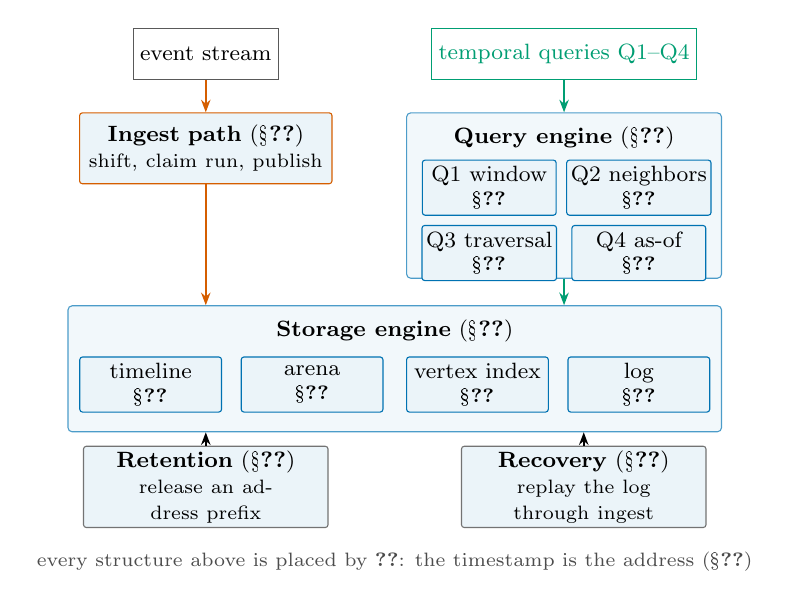
\begin{tikzpicture}[
  font=\footnotesize,
  comp/.style={draw=sysc, fill=sysc!8, rounded corners=1pt,
               minimum width=17mm, minimum height=7mm, inner sep=1.5pt,
               align=center, font=\footnotesize},
  grp/.style={draw=sysc!70, fill=sysc!5, rounded corners=1.5pt,
              inner sep=3pt},
  io/.style={draw=black!65, fill=white, minimum height=6.5mm,
             inner sep=2.5pt, align=center, font=\footnotesize},
  sub/.style={font=\scriptsize, text=black!70},
  fl/.style={-{Stealth[length=1.6mm]}, semithick},
]
% ---------------- inputs ----------------
\node[io] (stream) at (1.75, 4.25) {event stream};
\node[io, draw=qwin, text=qwin] (query) at (6.3, 4.25)
  {temporal queries Q1--Q4};

% ---------------- ingest path ----------------
\node[comp, draw=wins, text width=31mm, minimum height=9mm] (ingest) at (1.75, 3.05)
  {\textbf{Ingest path} (\S\ref{sec:storage-ingest})\\[0pt]
   {\scriptsize shift, claim run, publish}};
\draw[fl, wins] (stream) -- (ingest);

% ---------------- query engine ----------------
\node[grp, minimum width=40mm, minimum height=21mm] (qe) at (6.3, 2.45) {};
\node[anchor=north] at (6.3, 3.45) {\textbf{Query engine} (\S\ref{sec:query})};
\node[comp, minimum width=17mm] (qw) at (5.35, 2.55) {Q1 window\\[-1pt]{\scriptsize\S\ref{sec:query-window}}};
\node[comp, minimum width=17mm] (qx) at (7.25, 2.55) {Q2 neighbors\\[-1pt]{\scriptsize\S\ref{sec:query-expand}}};
\node[comp, minimum width=17mm] (qt) at (5.35, 1.72) {Q3 traversal\\[-1pt]{\scriptsize\S\ref{sec:query-traverse}}};
\node[comp, minimum width=17mm] (qa) at (7.25, 1.72) {Q4 as-of\\[-1pt]{\scriptsize\S\ref{sec:query-expand}}};
\draw[fl, qwin] (query) -- (qe.north);

% ---------------- storage engine ----------------
\node[grp, minimum width=83mm, minimum height=16mm] (se) at (4.15, 0.25) {};
\node[anchor=north] at (4.15, 1.0) {\textbf{Storage engine} (\S\ref{sec:storage})};
\node[comp, minimum width=18mm] (tl) at (1.05, 0.05)
  {timeline\\[-1pt]{\scriptsize\S\ref{sec:storage-tl}}};
\node[comp, minimum width=18mm] (ar) at (3.1, 0.05)
  {arena\\[-1pt]{\scriptsize\S\ref{sec:storage-tl}}};
\node[comp, minimum width=18mm] (vi) at (5.2, 0.05)
  {vertex index\\[-1pt]{\scriptsize\S\ref{sec:storage-vi}}};
\node[comp, minimum width=18mm] (wal) at (7.25, 0.05)
  {log\\[-1pt]{\scriptsize\S\ref{sec:storage-ret}}};
\draw[fl, wins] (ingest.south) -- (ingest.south |- se.north);
\draw[fl, qnbr] (qe.south) -- (qe.south |- se.north);

% ---------------- lifecycle operators ----------------
\node[comp, draw=black!55, text width=30mm, minimum height=9mm] (ret) at (1.75, -1.25)
  {\textbf{Retention} (\S\ref{sec:storage-ret})\\[0pt]
   {\scriptsize release an address prefix}};
\node[comp, draw=black!55, text width=30mm, minimum height=9mm] (rec) at (6.55, -1.25)
  {\textbf{Recovery} (\S\ref{sec:storage-ret})\\[0pt]
   {\scriptsize replay the log through ingest}};
\draw[fl] (ret.north) -- (ret.north |- se.south);
\draw[fl] (rec.north) -- (rec.north |- se.south);

% the abstraction underneath
\node[sub, anchor=north, align=center] at (4.15, -1.95)
  {every structure above is placed by \cref{eq:mapping}: the timestamp is the address (\S\ref{sec:tmap})};
\end{tikzpicture}
\caption{Engine components. Ingestion (\textcolor{wins}{vermillion})
writes, queries (\textcolor{qnbr}{green}) read; retention and
recovery act on the same four structures.}
\label{fig:overview}
\end{figure}


\subsection{Design Principle: The Temporal Address Space}
\label{sec:tmap}\label{sec:tmap-principle}
\texttt{mmap} turns a file range into an address range. \tmap turns a
\emph{time} range into an address range:
\begin{equation}
A(T) \;=\; A_{\mathrm{base}} + \big((T - T_{0}) \gg S\big)\times P,
\label{eq:mapping}
\end{equation}
one anonymous reservation in which the slot for time $T$ is a
subtraction and a shift away, for slot stride $P$ and granularity shift
$S$. A \emph{window} is the $2^S$ consecutive ticks of time that share
a slot, and a \emph{slot} is the address \cref{eq:mapping} assigns to
a window. The rest of \sys follows from this identity. We express the temporal
address space as five clauses. T1 is the basic placement rule: a
timestamp determines an address. T2 and T3 capture what this rule gains
from virtual memory: physical residency follows actual occupancy, and
time-based deletion becomes release of an address prefix. T4 and T5
specify the write discipline: append-only content makes recovery a
replay, while per-slot publication prevents readers from observing a
partial entry. Together, these clauses address the three challenges
from \S\ref{sec:intro}: T1 eliminates the time index, T5 provides
correct concurrent reads, and T2--T4 bound storage and simplify
retention and recovery. Any client that stores append-only records in
these slots can reuse the same guarantees.

\emph{T1 (Placement is arithmetic).} For any timestamp $t$, the slot
holding every event stamped $t$ is computed in $O(1)$ worst case with no
data-dependent memory access (Theorem~\ref{thm:addr}); there is no
search structure to consult, so the bound is unconditional.

\emph{T2 (Residency follows occupancy).} Resident memory is proportional
to \emph{occupied} time, not spanned time: a slot's page is faulted in
only when its window receives its first event, and untouched ranges cost
zero bytes whatever the virtual reservation (Theorem~\ref{thm:space}).

\emph{T3 (A time prefix is an address prefix).} Retention under a
time-based policy is a \texttt{madvise(}\allowbreak
\texttt{MADV\_DONTNEED)} over the address prefix
$[A_{\mathrm{base}}, A(t))$: whole pages return to the operating system,
readers of later windows are untouched, and no scan, tombstone, or
compaction is involved, because expiry order and address order coincide.

\emph{T4 (Content is a function of the appended multiset).} Slots
hold only what clients append, and nothing is updated in place, so
replaying an append log through the ordinary insert path reconstructs
the region exactly: recovery is re-ingestion
(Theorem~\ref{thm:recover}).

\emph{T5 (Per-slot publication).} A writer publishes an entry by storing
its payload first and its timestamp last with release semantics; fresh
pages read as zeros, and a zero timestamp marks an unpublished entry.
Readers acquire-load and skip, so no reader observes a torn or partial
entry during concurrent multi-writer ingestion
(Theorem~\ref{thm:conc}).

\emph{Scope of the Contract.} The clauses never mention edges: the
graph engine of \S\ref{sec:storage} is one client whose slots hold
pointers to edge blocks, and a per-window counter, a sketch, or a
key-value segment inherits the same five guarantees. The contract has
three limits. The granularity $S$ trades slot count against slot
occupancy and is bounded, not free (Theorem~\ref{thm:shift}); clause T5
gives per-entry atomicity, not multi-entry transactions; and nothing in
the contract helps a query keyed on anything other than time, which is
where the engine pays and \S\ref{sec:eval-structural} measures.

\subsection{Storage Engine}\label{sec:overview-storage}
Four components hold the stream. The \emph{timeline} is \tmap
instantiated with block pointers, one slot per window, so a window's
location is the arithmetic of \cref{eq:mapping} and nothing else. The
\emph{arena} is the bump-allocated region those blocks live in, holding
20-byte packed events that insertion never sorts. The \emph{vertex
index} is the per-vertex list of references into the arena that
answers the entity-keyed queries Q2 to Q4, the one structure a write
touches beyond the arena; each reference carries a copy of the event's
timestamp so that temporal predicates never read the arena. The
\emph{log} frames and checksums batches of raw events. Retention releases an address prefix, and recovery replays the log
through the ordinary insert path.

\subsection{Query Engine}\label{sec:overview-query}
Queries enter through one of two structures. Q1, the time-keyed
question, walks the timeline and reads blocks without consulting any
entity structure. Q2 and Q4, the entity-keyed questions, walk a
vertex's reference chain in the vertex index and reach the arena only
for references that pass the temporal predicate. Q3 composes Q2 under
a monotone time bound. \S\ref{sec:query} gives the processing and the
I/O behavior of each.

% Figure 3. Architecture on a live stream, with the formats strip merged in (was Figure 4): real structures with their real
% names, cell-level detail with example data, and the two example queries
% drawn as numbered colored steps ON the structures they touch. Two panels
% stacked so that every label is at least \scriptsize (7pt).
\begin{figure*}[t]
\centering
\tikzset{
  wstep/.style={circle, fill=wins, text=white, inner sep=0.25mm, font=\scriptsize\bfseries},
  bstep/.style={circle, fill=qwin, text=white, inner sep=0.25mm, font=\scriptsize\bfseries},
  gstep/.style={circle, fill=qnbr, text=white, inner sep=0.25mm, font=\scriptsize\bfseries},
}
\newcommand{\stepc}[2]{\tikz[baseline=-0.65ex]\node[#1]{#2};}
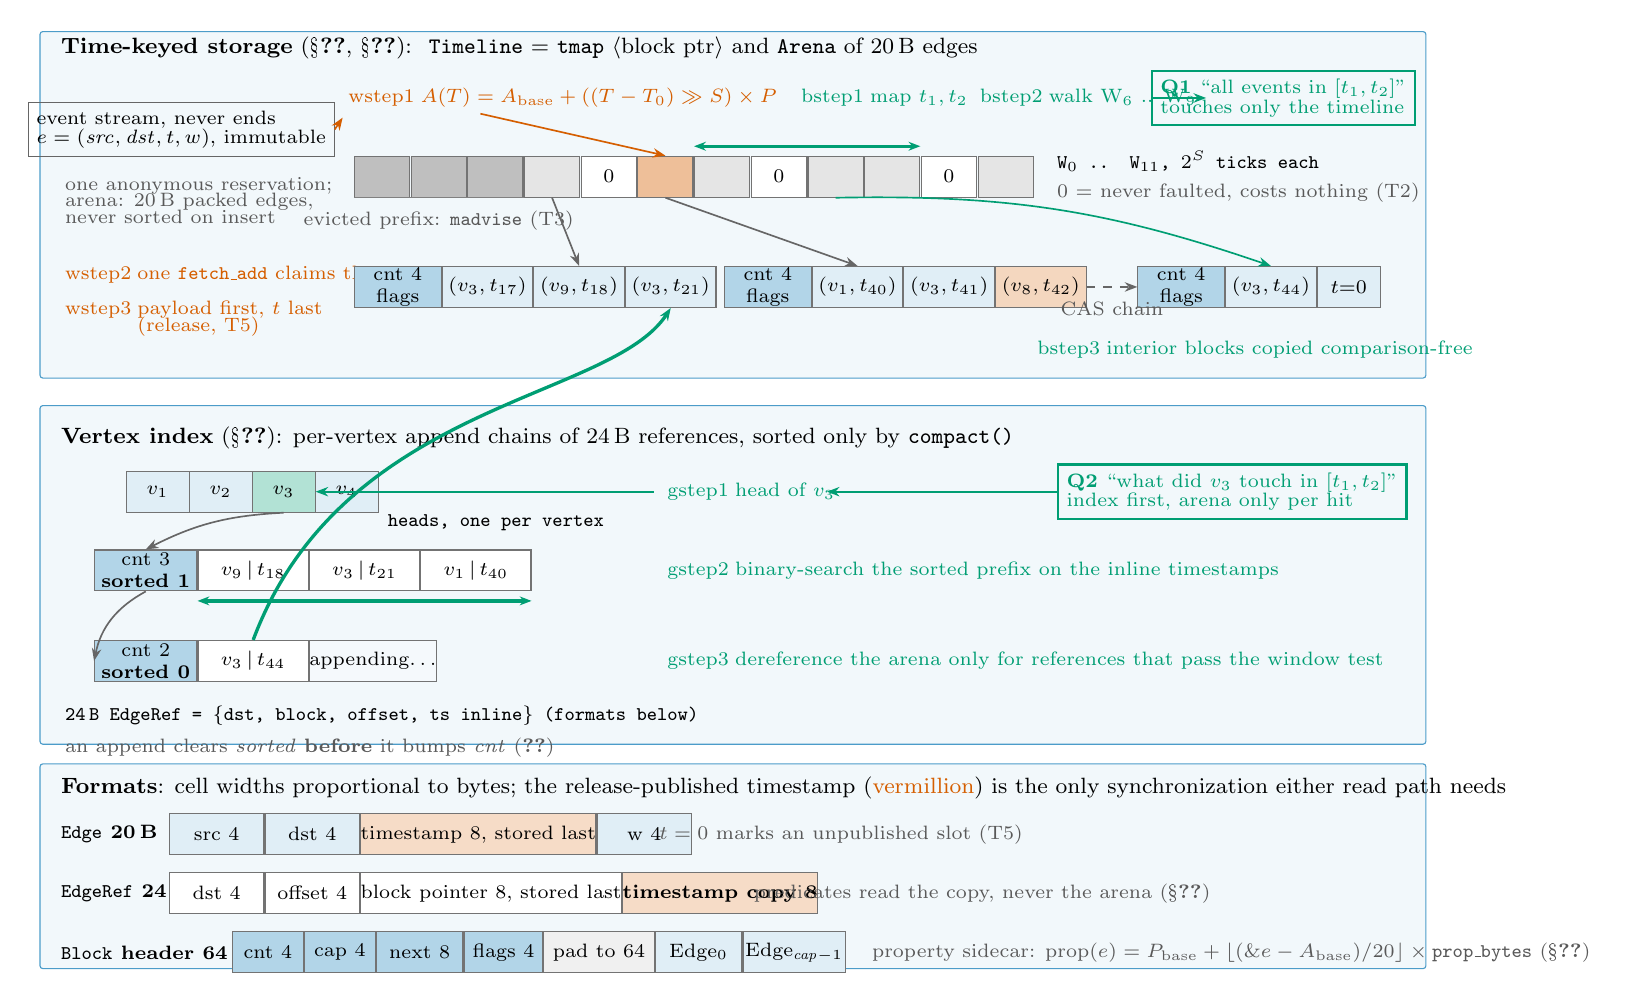
\begin{tikzpicture}[
  font=\footnotesize,
  panel/.style={draw=sysc!70, fill=sysc!5, rounded corners=1pt, inner sep=3pt},
  cell/.style={draw=black!55, inner sep=0pt, minimum height=5.2mm, font=\scriptsize},
  hdrc/.style={cell, fill=sysc!30},
  edgec/.style={cell, fill=sysc!12, minimum width=11.5mm},
  refc/.style={cell, fill=white, minimum width=14mm},
  slotc/.style={cell, minimum width=7mm},
  note/.style={font=\scriptsize, text=black!65},
  flow/.style={-{Stealth[length=1.6mm]}, semithick},
]

% ======================= Panel A: time-keyed storage ====================
\node[panel, minimum width=176mm, minimum height=44mm, anchor=north west] (pA) at (-0.25, 9.6) {};
\node[anchor=north west] at (-0.1, 9.65)
  {\textbf{Time-keyed storage} (\S\ref{sec:storage-tl}, \S\ref{sec:storage-ingest}):\;
   \texttt{Timeline} = \tmap$\langle$block ptr$\rangle$ and \texttt{Arena} of 20\,B edges};

% stream
\node[draw=black!60, inner sep=3pt, align=left, font=\scriptsize] (stream) at (1.55, 8.35)
  {event stream, never ends\\[-1pt] $e=(\mathit{src},\mathit{dst},t,w)$, immutable};
\node[note, anchor=west, align=left] at (-0.05, 7.45)
  {one anonymous reservation;\\[-2pt] arena: 20\,B packed edges,\\[-2pt] never sorted on insert};
\node[wins, font=\scriptsize, anchor=west] at (-0.05, 6.5)
  {\stepc{wstep}{2}\;one \texttt{fetch\_add} claims the run};
\node[wins, font=\scriptsize, anchor=west, align=left] at (-0.05, 5.95)
  {\stepc{wstep}{3}\;payload first, $t$ last\\[-2pt] \hphantom{\stepc{wstep}{3}\;}(release, T5)};

% insert step 1: the address computation
\node[wins, font=\scriptsize, anchor=west] (eq) at (3.55, 8.75)
  {\stepc{wstep}{1}\;$A(T)=A_{\mathrm{base}}+((T-T_0)\gg S)\times P$};
\draw[flow, wins] (stream.east) -- (3.6, 8.5);

% timeline slot array
\foreach \i/\f/\t in {0/black!25/, 1/black!25/, 2/black!25/, 3/black!10/, 4/white/0,
                      5/wins!40/, 6/black!10/, 7/white/0, 8/black!10/, 9/black!10/,
                      10/white/0, 11/black!10/}{
  \node[slotc, fill=\f] (s\i) at (4.1 + \i*0.72, 7.75) {\t};
}
\node[font=\scriptsize\ttfamily, anchor=west] at (12.55, 7.95) {W$_0$ .. W$_{11}$, $2^{S}$ ticks each};
\node[note, anchor=west] at (12.55, 7.55) {0 = never faulted, costs nothing (T2)};
\draw[black!50] (s0.south west) -- (s2.south east)
  node[midway, below=0.5mm, note, align=center] {evicted prefix: \texttt{madvise} (T3)};
\draw[flow, wins] (5.35, 8.55) -- (s5.north);

% arena blocks
\node[hdrc, minimum width=11mm] (b1h) at (4.3, 6.35) {\shortstack{cnt 4\\flags}};
\node[edgec, right=0mm of b1h] (b1e0) {$(v_3,t_{17})$};
\node[edgec, right=0mm of b1e0] (b1e1) {$(v_9,t_{18})$};
\node[edgec, right=0mm of b1e1] (b1e2) {$(v_3,t_{21})$};
\node[hdrc, minimum width=11mm] (b2h) at (9.0, 6.35) {\shortstack{cnt 4\\flags}};
\node[edgec, right=0mm of b2h] (b2e0) {$(v_1,t_{40})$};
\node[edgec, right=0mm of b2e0] (b2e1) {$(v_3,t_{41})$};
\node[edgec, fill=wins!25, right=0mm of b2e1] (b2e2) {$(v_8,t_{42})$};
\node[hdrc, minimum width=11mm] (b3h) at (14.25, 6.35) {\shortstack{cnt 4\\flags}};
\node[edgec, right=0mm of b3h] (b3e0) {$(v_3,t_{44})$};
\node[cell, fill=sysc!12, minimum width=8mm, right=0mm of b3e0] (b3e1) {$t{=}0$};
\draw[flow, black!60] (s3.south) -- (b1e1.north);
\draw[flow, black!60] (s5.south) -- (b2e0.north);
\draw[flow, black!60, dashed] (b2e2.east) -- (b3h.west)
  node[midway, below=0.6mm, note] {CAS chain};


% Q1 on the timeline
\node[draw=qwin, thick, inner sep=3pt, align=left, text=qwin, font=\scriptsize] (q1) at (15.55, 8.75)
  {\textbf{Q1} ``all events in $[t_1,t_2]$''\\[-1pt] touches only the timeline};
\draw[qwin, very thick, {Stealth[length=1.5mm]}-{Stealth[length=1.5mm]}]
  ([yshift=1.2mm]s6.north west) -- ([yshift=1.2mm]s9.north east);
\node[qwin, font=\scriptsize, anchor=west] (q1s) at (9.3, 8.75)
  {\stepc{bstep}{1}\;map $t_1,t_2$\;\;\stepc{bstep}{2}\;walk W$_6$ .. W$_9$};
\draw[flow, qwin] (q1.west) -- (q1s.east);
\node[qwin, font=\scriptsize, anchor=west] at (12.3, 5.55)
  {\stepc{bstep}{3}\;interior blocks copied comparison-free};
\draw[flow, qwin] (s8.south) to[bend left=10] (b3e0.north);

% ======================= Panel B: vertex index ==========================
\node[panel, minimum width=176mm, minimum height=43mm, anchor=north west] (pB) at (-0.25, 4.85) {};
\node[anchor=north west] at (-0.1, 4.7)
  {\textbf{Vertex index} (\S\ref{sec:storage-vi}): per-vertex append chains of 24\,B references,
   sorted only by \texttt{compact()}};

% head array
\foreach \i/\f in {1/sysc!12, 2/sysc!12, 3/qnbr!30, 4/sysc!12}{
  \node[cell, fill=\f, minimum width=8mm] (h\i) at (0.45 + \i*0.8, 3.75) {$v_{\i}$};
}
\node[font=\scriptsize\ttfamily, anchor=west] at (4.05, 3.35) {heads, one per vertex};

% bucket 1: sorted prefix
\node[hdrc, minimum width=13mm] (k1) at (1.1, 2.75) {\shortstack{cnt 3\\\textbf{sorted 1}}};
\node[refc, right=0mm of k1] (r1) {$v_9\,|\,t_{18}$};
\node[refc, right=0mm of r1] (r2) {$v_3\,|\,t_{21}$};
\node[refc, right=0mm of r2] (r3) {$v_1\,|\,t_{40}$};
% bucket 2: arrival-order tail
\node[hdrc, minimum width=13mm] (k2) at (1.1, 1.6) {\shortstack{cnt 2\\\textbf{sorted 0}}};
\node[refc, right=0mm of k2] (r4) {$v_3\,|\,t_{44}$};
\node[refc, fill=sysc!4, right=0mm of r4] (r5) {appending$\dots$};
\draw[flow, black!60] (h3.south) to[bend right=12] (k1.north);
\draw[flow, black!60] (k1.south) to[bend right=25] (k2.west);
\node[font=\scriptsize\ttfamily, anchor=west] at (-0.05, 0.9)
  {24\,B EdgeRef = \{dst, block, offset, \textbf{ts inline}\} (formats below)};
\node[note, anchor=west] at (-0.05, 0.5)
  {an append clears \emph{sorted} \textbf{before} it bumps \emph{cnt} (\cref{thm:conc})};

% Q2 on the index
\node[draw=qnbr, thick, inner sep=3pt, align=left, text=qnbr, font=\scriptsize] (q2) at (14.9, 3.75)
  {\textbf{Q2} ``what did $v_3$ touch in $[t_1,t_2]$''\\[-1pt] index first, arena only per hit};
\node[qnbr, font=\scriptsize, anchor=west] at (7.6, 3.75) {\stepc{gstep}{1}\;head of $v_3$};
\draw[flow, qnbr] (q2.west) -- (9.75, 3.75);
\draw[flow, qnbr] (7.55, 3.75) -- (h3.east);
\draw[qnbr, very thick, {Stealth[length=1.5mm]}-{Stealth[length=1.5mm]}]
  ([yshift=-1.2mm]k1.south east) -- ([yshift=-1.2mm]r3.south east);
\node[qnbr, font=\scriptsize, anchor=west] at (7.6, 2.75)
  {\stepc{gstep}{2}\;binary-search the sorted prefix on the inline timestamps};
\node[qnbr, font=\scriptsize, anchor=west] at (7.6, 1.6)
  {\stepc{gstep}{3}\;dereference the arena only for references that pass the window test};
\draw[flow, qnbr, very thick] (r4.north) .. controls (3.6, 4.9) and (7.0, 4.9) .. (b1e2.south);

% ======================= Panel C: formats ===============================
\node[panel, minimum width=176mm, minimum height=26mm, anchor=north west] (pC) at (-0.25, 0.3) {};
\node[anchor=north west] at (-0.1, 0.25)
  {\textbf{Formats}: cell widths proportional to bytes; the release-published timestamp (\textcolor{wins}{vermillion}) is the only synchronization either read path needs};
% Edge, 20 B at 3.0 mm/B
\node[font=\scriptsize\bfseries, anchor=west] at (-0.1, -0.60) {\texttt{Edge} 20\,B};
\node[cell, fill=sysc!12, minimum width=12mm] (fe1) at (2.0, -0.60) {src 4};
\node[cell, fill=sysc!12, minimum width=12mm, right=0mm of fe1] (fe2) {dst 4};
\node[cell, fill=wins!22, minimum width=24mm, right=0mm of fe2] (fe3) {timestamp 8, stored last};
\node[cell, fill=sysc!12, minimum width=12mm, right=0mm of fe3] (fe4) {w 4};
\node[note, anchor=west] at (7.5, -0.60) {$t=0$ marks an unpublished slot (T5)};
% EdgeRef, 24 B at 3.0 mm/B
\node[font=\scriptsize\bfseries, anchor=west] at (-0.1, -1.35) {\texttt{EdgeRef} 24\,B};
\node[cell, fill=white, minimum width=12mm] (fr1) at (2.0, -1.35) {dst 4};
\node[cell, fill=white, minimum width=12mm, right=0mm of fr1] (fr2) {offset 4};
\node[cell, fill=white, minimum width=24mm, right=0mm of fr2] (fr3) {block pointer 8, stored last};
\node[cell, fill=wins!22, minimum width=24mm, right=0mm of fr3] (fr4) {\textbf{timestamp copy 8}};
\node[note, anchor=west] at (8.7, -1.35) {predicates read the copy, never the arena (\S\ref{sec:storage-vi})};
% Block header, one 64 B line
\node[font=\scriptsize\bfseries, anchor=west] at (-0.1, -2.10) {\texttt{Block} header 64\,B};
\node[cell, fill=sysc!30, minimum width=9mm] (fh1) at (2.65, -2.10) {cnt 4};
\node[cell, fill=sysc!30, minimum width=9mm, right=0mm of fh1] (fh2) {cap 4};
\node[cell, fill=sysc!30, minimum width=11mm, right=0mm of fh2] (fh3) {next 8};
\node[cell, fill=sysc!30, minimum width=10mm, right=0mm of fh3] (fh4) {flags 4};
\node[cell, fill=black!6, minimum width=14mm, right=0mm of fh4] (fh5) {pad to 64};
\node[cell, fill=sysc!12, minimum width=11mm, right=0mm of fh5] (fh6) {Edge$_0$};
\node[cell, fill=sysc!12, minimum width=13mm, right=0mm of fh6] (fh7) {Edge$_{\mathit{cap}-1}$};
\node[note, anchor=west] at (10.2, -2.10)
  {property sidecar: $\mathrm{prop}(e) = P_{\mathrm{base}} + \lfloor (\&e - A_{\mathrm{base}})/20 \rfloor \times \texttt{prop\_bytes}$ (\S\ref{sec:storage-tl})};
\end{tikzpicture}
\caption{\sys architecture on a live stream: the structures, the two
queries of Example~\ref{ex:queries} drawn on them, and the formats.}
\label{fig:arch}
\end{figure*}


\begin{example}\label{ex:queries}
\cref{fig:arch} draws Q1 and Q2 on the structures of a live CADETS
stream. \textcolor{qwin}{\textbf{Q1}} (``all events in the last
hour'') maps both endpoints through \cref{eq:mapping}, walks the slots
between them, and copies interior blocks without comparisons.
\textcolor{qnbr}{\textbf{Q2}} (``what did process $v_3$ touch in that
hour'') walks $v_3$'s reference chain, binary-searches the sorted
prefix on the inline timestamps, and reaches the arena only for the
references that pass the window test. Neither consults an index that
ingestion maintains, because none exists.
\end{example}

% =====================================================================
\section{Storage Design}\label{sec:storage}
This section develops the write path. Three mechanisms sustain high-rate ingestion: arithmetic
placement, run-claiming publication, and compaction off the ingest
path. Retention and recovery then keep
storage bounded and reconstructible as the stream continues.

\subsection{Timeline and Arena}\label{sec:storage-tl}
\textbf{Key Idea.} Instantiate \tmap twice: a timeline of per-window
head pointers (\tmap slots are pointers), and an arena of
bump-allocated, cache-aligned edge blocks the pointers lead to. The
timeline inherits clauses T1--T3 directly; the arena holds 20-byte
packed edges and is never sorted on insert (\cref{fig:arch}, formats).

\begin{theorem}[Addressing]
\label{thm:addr}
For any timestamp $t$, the slot holding every edge stamped $t$ is
computed in $O(1)$ worst case, with no data-dependent memory access.
\end{theorem}
\begin{proof}
The map is one subtraction and one shift. Two timestamps land in the
same slot exactly when $\lfloor (t-T_0)/2^S \rfloor = \lfloor
(t'-T_0)/2^S \rfloor$, so every edge stamped $t$ is registered under
that one index and no other slot can hold one; no search structure is
consulted, so the bound is unconditional rather than expected-case.
\end{proof}

\begin{theorem}[Space]
\label{thm:space}
Let $P$ be the page size and $W_{occ}$ the number of non-empty
windows. Resident timeline memory is at most $W_{occ}\cdot P$ plus
page-table overhead the kernel materializes lazily; untouched windows
cost zero bytes, whatever the virtual reservation.
\end{theorem}
\begin{proof}
The timeline is an anonymous mapping of pointer slots. A page becomes
resident only when first written, and a slot is written only when its
window receives its first edge, so resident pages number at most the
pages holding an occupied slot, at most $W_{occ}$; untouched ranges
are never faulted in.
\end{proof}

Sparsity is absorbed by the memory management unit, not by a structure
the engine maintains; the mapping is anonymous, so the buffer-pool
failure modes of \S\ref{sec:background} never arise.

The shift $S$ sets how much time one slot covers. Too coarse and
windows overfill; too fine and the timeline sprawls. \sys picks $S$
from stream statistics (\cref{alg:shift}), and the choice is bounded.

\begin{algorithm}[t]
\small
\DontPrintSemicolon
\KwIn{event count $E$, span $L$, target occupancy $\tau$}
\KwOut{shift $S$}
$D \leftarrow \max(1, \lfloor E/\tau \rfloor)$ \tcp*{windows we want}
$w \leftarrow \max(1, \lfloor L/D \rfloor)$ \tcp*{width we want}
$S \leftarrow \lceil \log_2 w \rceil$ \tcp*{width we can address}
\Return{$S$}
\caption{\small Granularity selection.}
\label{alg:shift}
\end{algorithm}

\begin{theorem}[Granularity]
\label{thm:shift}
For $E \ge 2\tau$ events with target occupancy $\tau$, the selected
shift yields mean window occupancy $\mu \in [\tau/2,\, 4\tau)$.
\end{theorem}
\begin{proof}
The selector computes $D=\lfloor E/\tau \rfloor$ desired windows, a
desired width $w=\lfloor L/D \rfloor$, and takes the smallest $S$ with
$2^S \ge w$, so $2^S \in [w, 2w)$. The realized window count
$W=\lceil L/2^S \rceil$ then satisfies $D/2 < W \le D+1$, giving
$\mu = E/W \ge E/(D+1) \ge \tau/2$ and $\mu < 2E/D < 4\tau$.
\end{proof}

\cref{alg:shift} runs once on a stream prefix; re-running it on a
later prefix changes only future windows, because \cref{eq:mapping} is
evaluated per edge at insert time. The two factors of two in the bound
come from rounding the window width up to a power of two and from the
ceiling on the window count; across our datasets the bound holds at
per-window densities from 32 to 32{,}768 edges.

\subsection{Lock-Free Ingestion}\label{sec:storage-ingest}
\textbf{Key Idea.} Time-ordered arrival creates contention because
concurrent writers often target the same window. If every event
increments the same counter, that counter serializes the writers.
\sys therefore keeps the window counter as the only shared state,
protects readers through publication ordering rather than locks, and
amortizes the counter update across a run of events that share a
window.

An insert computes its slot (\cref{thm:addr}), claims an index in the
window's block with one \texttt{fetch\_add} on the block's counter, and
installs overflow blocks by compare-and-swap (CAS). Every failed CAS
means some other insert succeeded, so ingestion is lock-free and the
slot claim itself is wait-free. The insert path neither sorts nor rebalances data. Query correctness
therefore does not depend on arrival order, including when events
arrive late or out of order.

Readers are protected by a publication protocol instead of locks
(\cref{alg:publish}). A writer fills an edge's payload first and stores
its timestamp \emph{last} with release semantics. Fresh arena pages are
zero-filled, so a zero timestamp marks a slot that is not yet
published; readers acquire-load the timestamp and skip those. The
reference the writer then appends to the vertex index publishes the
same way, through its block pointer. One extra ordering rule makes the
fast read path safe as well: an append clears the \emph{sorted} flag
of the vertex-index bucket it lands in \emph{before} it bumps that
bucket's counter, so a reader that still sees the flag set knows that
no append has extended the prefix it is about to binary-search.

\begin{algorithm}[t]
\small
\DontPrintSemicolon
\SetKwProg{Fn}{}{}{}
\Fn{\textsc{Append}$(e)$}{
  $b \leftarrow$ arena block of slot $(e.t - T_0) \gg S$ \tcp*{\cref{thm:addr}}
  $i \leftarrow \textsc{FetchAdd}(b.\mathit{count}, 1)$ \hfill \textsf{(acq-rel)}\;
  \lIf{$i \ge b.\mathit{cap}$}{install overflow block by CAS; retry}
  write $e.\mathit{src}, e.\mathit{dst}, e.w$ into $b[i]$\;
  $b[i].t \leftarrow e.t$ \hfill \textsf{(release: publishes the edge)}\;
  $u \leftarrow$ tail bucket of $e.\mathit{src}$ in the vertex index\;
  $u.\mathit{sorted} \leftarrow \bot$ \hfill \textsf{(release)}\;
  $j \leftarrow \textsc{FetchAdd}(u.\mathit{count}, 1)$ \hfill \textsf{(acq-rel)}\;
  $u[j] \leftarrow (e.\mathit{dst}, i, e.t, b)$ \hfill \textsf{(block pointer last, release)}\;
}
\Fn{\textsc{Expand}$(v, t_{lo}, t_{hi})$}{
  \ForEach{bucket $u$ of $v$}{
    $n \leftarrow u.\mathit{count}$ \hfill \textsf{(acquire)}\;
    \lIf{$u.\mathit{sorted}$ \textsf{(acquire)}}{binary-search $u[0..n)$ on the inline $t$}
    \lElse{scan $u[0..n)$, skipping entries whose block pointer is $\bot$}
  }
}
\caption{\small Publication protocol.}
\label{alg:publish}
\end{algorithm}

\begin{theorem}[Concurrent reads]
\label{thm:conc}
Under this protocol no query observes a torn, partial, or unpublished
edge during concurrent multi-writer ingestion, and a reader that finds
the sorted flag set may binary-search the counted prefix.
\end{theorem}
\begin{proof}
For the first claim: a reader only accepts a slot whose timestamp is
non-zero, and the writer's release store of the timestamp happens
after its payload writes, so an acquiring reader that sees the
timestamp also sees the payload. A slot is written once and never
mutated, so no torn state exists after publication.

For the second: a reader loads the counter (acquire) and then the
flag. Suppose it observes the flag still set. Any append that could
have extended the counted prefix cleared the flag before bumping the
counter, and the reader's acquire on the counter synchronizes with
every bump it observes; so if any such bump were visible, the
corresponding clear would be visible too and the flag would be unset.
The observed prefix is therefore exactly the one compaction verified
and published, and binary search over it is sound.
\end{proof}

\textbf{Run Claiming.} Without further optimization,
\cref{alg:publish} performs one atomic read-modify-write per event.
When several writers target the same window, that counter becomes the
contended cache line. Run claiming amortizes this cost across multiple
events. Consecutive arrivals nearly
always share a window, so \texttt{insert\_batch} detects runs of
same-window events inside each thread's contiguous chunk and claims
each run with a single \texttt{fetch\_add} of the run length; the writer then fills the claimed slots with no
further synchronization, publishing each one as before. Overshooting a
block's capacity is benign because readers clamp to $\min(count,
capacity)$. \S\ref{sec:eval-analysis} isolates this effect. Without run claiming,
adding writers can reduce throughput because all writers contend on one
counter. With run claiming, ingestion scales to eight threads. When the
arrival order is fully shuffled and every run has length one, the
benefit disappears, confirming that the optimization exploits temporal
locality in the input stream.

\textbf{Consistency Model.} \sys provides per-edge atomic visibility:
once a reader observes an edge it observes it fully and forever
(\cref{thm:conc}), and a query's result is a subset of the edges
published before it completes. There are no multi-edge transactions
and no snapshot isolation: an append-only event stream has nothing to
isolate, and readers that want a fixed edge set take a static view
(\S\ref{sec:eval-structural}).

\subsection{The Vertex Index and the Compaction Contract}\label{sec:storage-vi}
\textbf{Key Idea.} The timeline answers ``what happened when''; it
cannot answer ``what did $v$ do'' without scanning every window. The
vertex index is the second structure, built beside the time-keyed store
rather than inside it: for each vertex, a chain of buckets holding
24-byte \emph{references} to that vertex's out-events in the arena,
each reference carrying a copy of the event's timestamp. Insertion
appends to the chain and never sorts it; only an explicit
\texttt{compact()} pass ever does, so the write path never pays for the
read path's ordering.

Appends leave a vertex's neighborhood in arrival order, so a
time-windowed expansion has to scan it: $O(d)$ for out-degree $d$. An
explicit \texttt{compact()} pass sorts each neighborhood by timestamp
once, and afterwards expansion binary-searches in $O(\log d + k)$ for
$k$ results. Compaction is not on the insert path: compacting after every
batch re-walks the whole index, the same $O(\text{index})$-per-batch
cost a sorted structure pays by design.

Queries are correct before and after compaction; compaction changes
performance, not semantics. This yields a central trade-off. A
statically sorted structure obtains fast temporal expansion by making
sorting mandatory, which requires rebuilding before new data is fully
integrated. \sys keeps sorting off the ingest path, so it remains
appendable and queryable during ingestion; an explicit compaction can
later restore the faster binary-search path when convenient.

\textbf{Discussion.} Each entry is \texttt{EdgeRef} $=$
\{\texttt{dst}, \texttt{offset}, \texttt{block}, \texttt{ts}\}, 24
bytes; the 8-byte timestamp copy is what lets a temporal predicate be
tested from one contiguous stream instead of one random arena read per
candidate, and \S\ref{sec:eval-analysis} prices it on both sides.

\subsection{Retention and Durability}\label{sec:storage-ret}
\label{sec:design-durability}
\textbf{Key Idea.} Retention is forgetting, deleting every event older
than a horizon while the stream keeps arriving; durability is
reconstructing the store after a crash from what reached stable
storage. A vertex-keyed layout scatters the expired events across
every neighborhood and must checkpoint its index; under
\cref{eq:mapping} both become operations on the address space.

Retention is a monotone predicate on time, so it is an operation on
an address prefix. \texttt{evict\_before($t$)} walks the timeline
prefix, merges the block extents it finds, and returns whole pages to
the operating system with \texttt{madvise}; readers of other windows
are untouched. There is no scan of the edge set and no tombstone
compaction, because expiry and address order coincide.

Durability uses a property most databases do not have: engine state is
a pure function of the edge multiset, because edges are immutable and
deletion is retention policy rather than semantics. The log is
therefore framed, checksummed batches of raw edges, written by an
asynchronous thread that overlaps insertion, and recovery is replaying
it through the ordinary insert path, with no undo or redo
phase~\cite{mohan1992aries} and no idempotence bookkeeping; a torn tail frame fails its length or
checksum test and is discarded.

\begin{theorem}[Recovery]
\label{thm:recover}
Replaying the durable log prefix through the ordinary insert path
yields an engine state answering every query identically to the
pre-crash state restricted to logged edges.
\end{theorem}
\begin{proof}
Engine state is a function of the inserted multiset only: insertion
consults no clock, no random source, and no cross-edge state beyond
allocation order, and query results are independent of intra-window
physical order because uncompacted reads scan whole windows and
compaction sorts them into one canonical order. The replayed multiset
equals the logged multiset by the frame checksums, so both states
answer alike. Fault injection in \S\ref{sec:eval-recovery} tests the
claim: 50 crash points and 60 torn-tail corruptions, zero divergences.
\end{proof}

% =====================================================================
\section{Temporal Query Engine}\label{sec:query}
The query engine is designed around the same priority as the storage
engine: sustain the incoming stream, then expose the temporal operators
required by the target workload. It implements the four queries in
\cref{tab:queries}, each by scanning the structure whose organization
matches the query key. Every operator remains correct before and after
compaction (\cref{thm:conc}). Higher-level query languages,
optimization, and general graph-analytics kernels are outside the
storage layer; for those workloads, \sys exports a static view
(\S\ref{sec:eval-structural}). \cref{tab:complexity} collects the
bounds.

\subsection{Query Processing on the Timeline}\label{sec:query-window}
Q1, \texttt{query\_range}$(t_1,t_2)$, maps both endpoints through
\cref{eq:mapping} and walks the slots between them. Interior slots lie
entirely inside the window, so their blocks are copied out
\emph{comparison-free}; only the two boundary slots filter per edge,
and a block whose fill compaction has verified skips even the per-edge
publication check. The walk touches $W$ pointer slots and the $O(W\mu)$
edges under them, all sequentially, so the cost is $O(W + W\mu + |R|)$
with no per-edge pointer chase. \texttt{window\_aggregate\_sum} runs
the same walk without materializing edges.

\subsection{Query Processing on the Vertex Index}\label{sec:query-expand}
Q2, \texttt{neighbors}$(v, t_1, t_2)$, walks $v$'s reference chain.
A bucket whose sorted flag is set (\cref{alg:publish}) is
binary-searched for the window's lower bound and scanned to its upper
bound, $O(\log d + k)$; a bucket whose flag is clear is scanned whole
with unpublished entries skipped, $O(d)$. Because each reference
carries a copy of the timestamp (\S\ref{sec:storage-vi}), both paths
read one contiguous 24-byte-stride stream and touch the arena only for
the $k$ delivered edges, never per candidate; this copy is what made
uncompacted expansion up to $5.5\times$ faster, and it is what a store
keyed only on time cannot do at all (\S\ref{sec:eval-temporal}).

\textbf{As-of Retrieval.} Q4 asks for the neighborhood of $v$ as it
stood at time $t$: for each distinct neighbor, the latest event up to
$t$. A versioned store keeps one current version per pair and answers
in one step; an event store keeps every event and must reduce them.
\cref{alg:asof} does so from the same chain: a sorted bucket stops at
the first reference past $t$, an unsorted one is filtered whole, and a
flat sort on $(peer \uparrow, ts \downarrow)$ keeps the head of each
run with no hash table. The cost is $O(d_{\le t}\log d_{\le t})$
against $O(d_{\mathit{distinct}})$ for a version-grouped store, and
\S\ref{sec:eval-temporal} prices that difference.

\begin{algorithm}[t]
\small
\DontPrintSemicolon
\SetKwProg{Fn}{}{}{}
\Fn{\textsc{LatestNeighbors}$(v, t)$}{
  $R \leftarrow \emptyset$\;
  \ForEach{bucket $u$ of $v$}{
    $n \leftarrow u.\mathit{count}$, $s \leftarrow u.\mathit{sorted}$ \hfill \textsf{(acquire)}\;
    \For{$i \leftarrow 0$ \KwTo $n-1$}{
      \lIf{$u[i].\mathit{block} = \bot$ \textsf{(acquire)}}{\textbf{continue}}
      \lIf{$u[i].ts > t$}{\textbf{break} if $s$, else \textbf{continue}}
      append $(u[i].\mathit{dst},\, u[i].ts)$ to $R$\;
    }
  }
  sort $R$ by $(\mathit{peer}\uparrow,\, ts\downarrow)$\;
  \Return{head of each $\mathit{peer}$ run of $R$}\;
}
\caption{\small As-of retrieval (Q4).}
\label{alg:asof}
\end{algorithm}

\subsection{Time-Respecting Traversal}\label{sec:query-traverse}
Q3 composes Q2 under a monotone time bound, and it is the query of
\cref{fig:motivation}. \texttt{forward\_taint}$(s, t_s, t_{hi})$
labels every vertex reachable from $(s,t_s)$ along non-decreasing
timestamps in $[t_s,t_{hi}]$ with the \emph{earliest} time it could
have become tainted, the forward question of \cref{ex:cadets};
\texttt{backward\_trace} is its mirror over in-edges, the backward
question. Both run temporal Dijkstra: a priority queue keyed on
arrival time, where relaxing a vertex expands only the suffix of its
neighborhood beyond the frontier time, exactly the suffix a sorted
bucket binary-searches to. Cost is $O(\sum_{v \in R}(\log d(v) + k_v)
+ |R|\log|R|)$ over \emph{reached} vertices only, never $O(V)$: the
time bound prunes at the bucket level, before any arena access, which
is why the attack chain of \cref{fig:motivation} reconstructs inside
an impact set that is a tiny fraction of the graph
(\S\ref{sec:eval-temporal}).

\begin{table}[t]
\caption{\small Time complexity of core operations.}
\label{tab:complexity}
\scriptsize
\setlength{\tabcolsep}{2.5pt}
\begin{tabular}{@{}llll@{}}
\toprule
Operation & \sys compacted & uncompacted & time-sorted CSR \\
\midrule
append one edge      & $O(1)$ am.                 & same        & $O(E)$ rebuild \\
Q1 range $[t_1,t_2]$ & $O(W+W\mu+|R|)$            & same        & $O(V\log d+|R|)$ \\
Q2 expand $v$        & $O(\log d(v)+k)$           & $O(d(v))$   & $O(\log d(v)+k)$ \\
Q3 traversal         & $O(\sum\log d+|R|\log|R|)$ & $O(\sum d+\cdots)$ & as compacted \\
Q4 as-of             & $O(d_{\le t}\log d_{\le t})$ & same      & same \\
\texttt{evict\_before} & $O(W_{ev}+\text{blocks})$ & same       & $O(E)$ rebuild \\
\texttt{compact}     & $O(E\log B_{\max})$ optional & --         & $O(E\log E)$ mandatory \\
\bottomrule
\end{tabular}
\par\smallskip\scriptsize
$E$ events, $V$ vertices, $d(v)$ out-degree, $\mu$ window occupancy
(Thm.~\ref{thm:shift}), $W$ windows in a range, $|R|$ result size, $k$
results per expansion, $B_{\max}$ the largest bucket.
\end{table}

% =====================================================================
\section{Implementation}\label{sec:impl}
\sys is implemented in C++17 with no dependencies beyond the standard
library and POSIX \texttt{mmap}/\texttt{madvise}. Once \tmap removes the conventional time index and simplifies
allocation and recovery, the remaining implementation choices are
mostly hardware-facing. This section describes five such choices and
why each matters.

\emph{Virtual Memory as the Allocator.} The engine performs no
\texttt{malloc} on the write path. The timeline and the arena are two
anonymous reservations sized from the stream's span, its expected
volume, and its vertex count, mapped with \texttt{MAP\_NORESERVE} so
that a reservation larger than physical memory is accepted and only
touched pages are ever charged; a page fault on first touch is the only
allocation, and
\texttt{madvise(MADV\_DONTNEED)} is the only free. The one hardware
knob that interacts with this choice is the page size. Transparent
huge pages (THP)~\cite{kwon2016ingens} replace a 4\,KB fault by a 2\,MB one, and on a sparse
timeline a window that holds a handful of events then costs 2\,MB of
resident memory, which defeats clause T2: on the dataset that motivated
the experiment THP cost $28\%$ of ingestion throughput and $69\%$ more
resident memory, so the engine disables it on its mappings.

\emph{Cache-Line Layout.} An arena block starts with a 64-byte header
that holds the counter writers contend for, its capacity, the overflow
pointer, and the flags; nothing else shares that line, so contention
on the counter never evicts payload. Edges are packed to 20 bytes with
no padding, so a window scan reads 3.2 edges per line fetched. A
vertex-index reference is 24 bytes, of which 8 are the timestamp copy
that keeps the temporal predicates of Q2 to Q4 on a sequential stream
instead of one random DRAM access per candidate.

\emph{Atomics and Memory Ordering.} The write path uses three atomic
operations and no fence instructions: a \texttt{fetch\_add} with
acquire-release ordering on a block or bucket counter, a CAS on an
overflow pointer, and a release store of the timestamp (arena) or the
block pointer (vertex index) that publishes an entry. Readers use
acquire loads. On the x86 total-store-order memory model~\cite{sewell2010x86tso} a release
store and an acquire load compile to plain moves, so the protocol's
only cost is the read-modify-write on the counter, and that is the
cost run claiming amortizes over a run. On a weaker memory model the
same code is correct and the release stores become real barriers.

\emph{SIMD Boundary Filter.} Only the two boundary slots of a Q1 range
compare timestamps, which invites vectorization: an AVX2 gather path
filters eight timestamps per iteration. Across four datasets and five
window widths it never won, because a 64-bit gather at a 20-byte
stride is slower than scalar loads and a range scan only ever filters
its two boundary slots; it ships disabled.

\emph{The Log and the Storage Device.} The log writer frames each
insert batch with a length and a checksum and appends it from a
dedicated thread, so ingestion runs at memory speed while the log
trails. The \texttt{fsync} policy is the operator's knob: from an
asynchronous 4\,MB group commit onward the durable ingestion rate is
bounded by the device's sequential write bandwidth, not by the engine
(\S\ref{sec:eval-recovery}), and acknowledgment after group commit is
the intended deployment. Recovery is replay through
\texttt{insert\_batch} itself, so every line of the recovery path is
exercised by every ordinary ingest.

% =====================================================================
\section{Evaluation}\label{sec:eval}
The evaluation asks three questions. First, how quickly can \sys
ingest an event stream relative to competing stores? Second, how well
does its time-keyed layout support the four temporal queries in
\cref{tab:queries}? Third, what is the cost of this layout for
structural analytics that ignore time? We answer these questions under
a common protocol across four datasets. Across the temporal
experiments, \sys wins 59 of 64 comparisons; the five losses are
reported and explained below.

\subsection{Experiment Setup}\label{sec:eval-setup}
\textbf{Hardware.} One machine: a 10-core Intel Xeon W-2255 (20
hardware threads, 3.7\,GHz), 188\,GB of memory, a 2\,TB SATA hard
disk (7{,}200\,rpm) that holds the datasets and the logs, Ubuntu 20.04.
All systems run in the same process or on the same machine, with eight
worker threads unless a system's own write path is single-threaded,
which the text notes.

\textbf{Datasets.} Four event datasets, large to small, chosen to span
three orders of magnitude of volume and the three workload families of
\S\ref{sec:intro} (\cref{tab:breadth}). LANL is 58 days of enterprise
authentication events from the Los Alamos National Laboratory
network~\cite{lanl2015data}, the largest public event graph we know of
at 1.05 billion events over 18K hosts. THEIA and CADETS are whole-system
provenance traces from the DARPA Transparent Computing
program~\cite{darpa2020tc}, Linux and FreeBSD hosts respectively, with
documented intrusions inside (\cref{ex:cadets}). wiki-talk is the
Wikipedia user-talk interaction stream from SNAP~\cite{leskovec2014snap, paranjape2017motifs}
and the dataset TVA's own evaluation uses. Every result in this section
is on these four; the \sys-only measurements were also run on eleven
further public datasets, including LDBC-SNB~\cite{erling2015ldbc} at
scale factor~10, with the same conclusions.

\begin{table}[t]
\centering\footnotesize
\setlength{\tabcolsep}{4pt}
\caption{Datasets.}
\label{tab:breadth}
\begin{tabular}{@{}llrrrl@{}}
\toprule
Dataset & Family & Events & $|V|$ & Span & Source \\
\midrule
LANL      & authentication telemetry & 1.05B & 18K  & 58 d  & \cite{lanl2015data} \\
THEIA     & system provenance        & 97.3M & 6.9M & 10 d  & \cite{darpa2020tc} \\
CADETS    & system provenance        & 22.5M & 2.9M & 11 d  & \cite{darpa2020tc} \\
wiki-talk & interaction stream       & 7.8M  & 1.1M & 6.4 y & \cite{leskovec2014snap} \\
\bottomrule
\end{tabular}
\end{table}


\textbf{Competitors.} Seven systems, each run through its own fastest
documented path. GraphOne~\cite{kumar2019graphone} and
LiveGraph~\cite{zhu2020livegraph} are streaming graph stores that
absorb an edge stream alongside analytics, key storage on the source
vertex, and carry the timestamp as an edge property.
Stinger~\cite{ediger2012stinger} and Sortledton~\cite{fuchs2023sortledton}
are structural dynamic graph stores that key edges on the $(src,dst)$
pair and treat a repeated pair as an update, so they answer the
ingestion question but not Q1 to Q4 over an event multiset.
RocksDB~\cite{dong2021rocksdb} is the key-value store, given a
big-endian \texttt{ts:src:}\allowbreak\texttt{dst:seq} key so that a
time range is one contiguous key range, the schema TVA's own disk
backend uses. DuckDB~\cite{raasveldt2019duckdb} is the columnar engine,
given indexes on \texttt{ts} and \texttt{(src,ts)}.
TVA~\cite{li2026tva} is the versioned temporal graph store. All are
built from source and driven in-process except GraphOne, driven through
its own harness with our query jobs added. A time-sorted static CSR,
which cannot ingest, appears as a reference where informative.

\textbf{Queries and Measurement.} The query set is \cref{tab:queries},
with a window width of 1\% of the dataset span; Q1 is the trailing
window, and Q2 to Q4 use 1{,}000 queries per dataset drawn uniformly
over events, so that each targets an entity at a time it was active,
handed to every system in the same order. Every system's answer is
compared element-wise against \sys's through a checksum over the
delivered edges, vertices, or pairs before any latency is reported;
every number in this section passed. We report medians with tails,
never means. A query phase that would exceed 15 minutes on a system
is cut after a prefix of the queries and marked; an ingestion that
does not finish in 90 minutes is reported with the rate it sustained.

\textbf{Configuration.} Every mechanism this paper analyzes ships as a
switch in \sys's configuration, and the measured defaults are used
throughout: run claiming on, the binary-search threshold 32, the SIMD
scan and transparent huge pages off, the inline timestamp on. The
property sidecar and the reverse index are attached only where a
measurement needs them, and \S\ref{sec:eval-analysis} prices each.
Our artifact is available at
\url{https://anonymous.4open.science/r/TGSA-5D74/}.

\begin{figure*}[t]
  \centering
  \includegraphics[width=0.95\textwidth]{figures/fig_ingest.pdf}
  \caption{\small Ingestion. (a) Events per second on eight threads. (b) The
  same while four readers query the store. (c) Resident bytes per
  event after ingestion.}\vspace{-2ex}
  \label{fig:ingest}
\end{figure*}

\subsection{Ingestion Throughput}\label{sec:eval-ingest}
\cref{fig:ingest}(a) shows that \sys sustains the highest ingestion
rate on three of the four datasets and is effectively tied with
GraphOne on THEIA. It reaches 72.5M events/s on LANL, 60.3M on CADETS,
54.2M on wiki-talk, and 33.3M on THEIA. Relative to GraphOne, the
fastest competitor, this is $1.6$ to $1.9\times$ faster on three
datasets and a near tie on THEIA ($33.3$ versus $34.8$M). The gap to
the remaining systems is larger: $4$ to $13\times$ over LiveGraph,
$11$ to $39\times$ over RocksDB and DuckDB, and $20$ to
$2{,}400\times$ over Sortledton and Stinger.

The comparison uses the same event order and 64K-event batches for
every system and includes all work required before the new data can be
queried correctly: publication in \sys, archival into GraphOne's
adjacency, RocksDB's memtable flush, and DuckDB's index construction.
THEIA is the only dataset on which \sys does not lead. Its 64K-event
batches are split across eight threads while updates are spread over a
6.9M-vertex index, which shortens same-window runs and therefore reduces
the benefit of run claiming. Supplying THEIA as one batch raises \sys
to 79M events/s; across all four datasets, the corresponding one-batch
ceiling is \nSingleCallLo{} to \nSingleCallHi{}M events/s
(\S\ref{sec:eval-analysis}). Every competitor finished the
billion-event dataset within the budget.

\textbf{Streaming graph stores.} GraphOne is the closest competitor
because, like \sys, it absorbs events through a memory-speed log before
organizing them for graph access. Its archive thread keeps pace at
$31$ to $41$M events/s and matches \sys on THEIA, where both systems
are dominated by per-vertex work. LiveGraph's fastest path is its bulk
loader, at $4.9$ to $7.9$M events/s. Each append must first locate the
relevant version chain, which limits throughput; its transactional path
is slower still (\S\ref{sec:eval-concurrent}).

\textbf{Structural graph stores.} Stinger and Sortledton are slower
because their data model treats a repeated $(src,dst)$ pair as an
update rather than a new event. Each repeated contact must therefore
locate the existing edge inside its neighborhood, and the cost grows
with both pair multiplicity and neighborhood length. Stinger sustains
$1.4$M events/s on LANL, which contains only 420K distinct pairs, but
falls to $0.02$M on CADETS, where hot processes accumulate millions
of events. Sortledton, evaluated on the deduplicated pair stream (with
deduplication charged to the collector rather than the store), sustains
$1.2$ to $2.9$M pairs/s. Neither system can preserve the original
event multiset on a round trip.

\textbf{Key-value and columnar engines.} We configure both systems to
favor temporal access. RocksDB receives a time-encoded key, producing
a sequential write pattern that is close to the best case for an LSM
store. Even so, it ingests $11$ to $38\times$ slower than \sys because
each event is written to the log, the memtable, and again during
merges. In DuckDB, maintaining the two query indexes costs more than
the base load at every dataset size.

\textbf{Versioned temporal graph store.} TVA illustrates the cost of
using version chains for an event-multiset workload. It did not finish
wiki-talk's 7.8M events within the 90-minute cutoff (terminated at
5{,}415\,s with 41.6\,GB resident memory while remaining CPU-bound),
which bounds its rate below 1{,}447 events/s. TVA maintains a version
chain for each $(src,dst)$ pair; in an event stream, the chain length
therefore grows with pair multiplicity, contrary to its intended
few-versions-per-entity regime. This is a workload mismatch rather
than a universal disadvantage: \S\ref{sec:eval-temporal} shows the
query for which TVA's version-oriented design is preferable.

\textbf{Ingestion under Concurrent Queries.}\label{sec:eval-concurrent}
A streaming store must continue to ingest while queries are running.
We therefore preload half of each dataset, stream the remainder through
eight writers at full speed, and concurrently run four Q2 readers over
settled windows. Every answer is checked against a quiescent reference.
Under this mixed workload, \cref{fig:ingest}(b) shows that \sys
sustains $57.9$ to $74.0$M events/s, $3.0$ to $4.7\times$ GraphOne and
$3.6$ to $10.7\times$ LiveGraph.

Query throughput shows the complementary trade-off. \sys serves
$3.0\times$ more queries per second than GraphOne on wiki-talk, whereas
GraphOne is $1.5$ to $2.5\times$ faster on the three datasets whose
sampled Q2 queries frequently hit hub vertices; \S\ref{sec:eval-temporal}
explains the same effect for THEIA. Across all runs, the mismatch count
is zero. LiveGraph is competitive only after the collector repartitions
the stream by source vertex. With the original arrival order, its
vertex-locked transactions fall from 1.75M events/s with one writer to
0.01M with eight writers and incur 209K aborts.

\textbf{Storage consumption.} The time-keyed layout does not require a
large space premium (\cref{fig:ingest}(c)). Including the vertex index
and copied timestamps, \sys uses $44$ to $58$ resident bytes per
20-byte event. This is the lowest footprint on THEIA, CADETS, and
wiki-talk, and is within $25\%$ of GraphOne's 35 bytes on LANL, where
only 18K vertices make GraphOne's per-vertex overhead negligible.
LiveGraph uses $84$ to $97$ bytes per event, while DuckDB uses $49$ to
$116$ with its two indexes. Stinger and Sortledton are omitted because
they store one edge per distinct pair rather than the full event
multiset.

\begin{figure*}[t]
  \centering
  \includegraphics[width=0.9\textwidth]{figures/fig_queries.pdf}
  \caption{\small Temporal queries Q1 to Q4 (rows) on the four datasets
  (columns), every answer verified against \sys's. A missing bar is a
  query the system cannot express; a bar marked with a fraction is the
  prefix the system completed within the budget.}\vspace{-2ex}
  \label{fig:queries}
\end{figure*}

\subsection{Temporal Query Performance}\label{sec:eval-temporal}
\cref{fig:queries} compares all four temporal queries on all four
datasets. The result is consistent across query types: \sys wins every
Q1 and Q3 comparison and most Q2 and Q4 comparisons. Its losses occur
when Q2 or Q4 targets very high-degree vertices, where a vertex-grouped
layout has an advantage. Each row uses a shared vertical scale so that
the magnitude of these differences can be compared across datasets.

\textbf{Q1, window scan.} Q1 directly tests the benefit of making time
the physical address. \sys answers a 1\% window in $0.9$\,ms on
wiki-talk and $81$\,ms on LANL, where the query returns 13.3M events.
It is $3.2$ to $13.5\times$ faster than DuckDB and $23$ to $69\times$
faster than RocksDB, although both are configured for temporal
access. \sys is faster because
the window is already a contiguous address range and interior slots
can be copied without a timestamp comparison per event.

The contrast is larger for vertex-keyed stores. GraphOne is $3.3$ to
$19\times$ slower and LiveGraph $80$ to $242\times$ slower because
they must search across neighborhoods to recover events from a global
time window.

\textbf{Q2, windowed neighbors.} Q2 favors vertex-keyed layouts, so it
is the closest temporal comparison. \sys answers at a median of
$1.7$ to $77$\,$\mu$s. It is $4.3$ to $92\times$ faster than LiveGraph,
which scans the full neighborhood and tests each edge, and $30$ to
$528\times$ faster than DuckDB. RocksDB is $1{,}150$ to $41{,}000\times$ slower
because its time-first key forces it to scan the entire query window
and then filter by source.

\sys is $1.9$ to
$27\times$ faster on LANL, CADETS, and wiki-talk, but GraphOne is
$1.5\times$ faster on THEIA. The reason is not temporal filtering but
hub structure: sampled THEIA queries often target processes with
millions of events. Their \sys reference chains span roughly twenty
geometrically growing buckets, each of which must be binary-searched,
whereas GraphOne keeps one archived adjacency array per vertex. This
outlier identifies a concrete optimization opportunity: storing a time
range per bucket would let \sys skip buckets that cannot overlap the
query window.

\textbf{Q3, time-respecting traversal.} Q3 tests whether the Q2 access
advantage composes across multiple hops. \sys answers at a median of
$0.47$\,ms on CADETS to $43$\,ms on THEIA. GraphOne is $1.5$ to
$16\times$ slower and LiveGraph $3.6$ to $77\times$ slower. DuckDB
pays a scan at each hop and is $35$ to $1{,}500\times$ slower on the
prefix it completes; RocksDB finishes between zero and 44 of the
1{,}000 traversals within the time budget.

The attack chain in \cref{fig:motivation} provides a concrete example.
Starting from the implant, \sys reconstructs the published forward
chain in 133\,$\mu$s while visiting an impact set equal to only
0.0093\% of the graph; tracing backward from the alert isolates the
same chain. The temporal bound prunes expansion at the bucket level before
the arena is touched, so cost follows the reachable region, not the
graph.

\textbf{Q4, as-of neighbors.} Q4 is the query for which a
version-oriented representation has the clearest structural advantage.
A store that maintains one current version per $(v,u)$ works in time
proportional to the number of distinct neighbors, whereas an event
store must reduce all events up to $t$. Even with this disadvantage,
\sys answers at a median of $23$\,$\mu$s on wiki-talk to $9.2$\,ms on
LANL. It is $1.25$ to $1.8\times$ faster than LiveGraph and $1.3$ to
$81\times$ faster than DuckDB on every dataset. Against GraphOne, \sys
is faster on CADETS and wiki-talk ($1.2$ and $3.0\times$) but slower on
THEIA and LANL ($2.8$ and $4.7\times$).

The two losses are again caused by hubs, but here the cost is in the
reduction rather than the search. \cref{alg:asof} sorts surviving
references by neighbor, which is $O(d\log d)$ for a hub with millions
of events, while GraphOne uses a hash-based $O(d)$ reduction, the asymptotic advantage of a
version-grouped representation stated in \S\ref{sec:query-expand}.

\begin{figure}[t]
  \centering
  \includegraphics[width=0.95\linewidth]{figures/fig_analytics.pdf}
  \caption{\small Analytics on the stored graph. (a) The extract-to-analytics
  pipeline end to end at the 1\% window. (b) Whole-graph BFS, time
  ignored, identical algorithm code over each layout.}\vspace{-2ex}
  \label{fig:analytics}
\end{figure}

\textbf{End-to-end analytics.} We next ask whether faster temporal
extraction matters once an analytics computation is included. The
pipeline extracts a window, builds the algorithm's working structure,
runs ten PageRank rounds or label propagation to convergence, and
writes the per-vertex result back. The compute code is identical for
all stores, so differences come from the storage-facing stages.

At the 1\% window, \cref{fig:analytics}(a) shows that \sys is $1.1$ to
$1.6\times$ faster than DuckDB end to end and $4.7$ to $12\times$
faster than LiveGraph; 0.1\% and 10\% windows preserve the same
ordering. The breakdown explains why: extraction consumes $85$ to
$96\%$ of LiveGraph's pipeline and $42$ to $71\%$ of DuckDB's, but
only $36$ to $54\%$ of \sys's. With extraction reduced, the identical
compute phase becomes the dominant share.

\subsection{Structural Workloads}\label{sec:eval-structural}
Structural analytics deliberately ignore the dimension around which
\sys is organized, so this experiment measures the price of the
layout's specialization. We run identical BFS, PageRank, and label
propagation code over adjacency supplied by each store and require
checksum-identical results. \cref{fig:analytics}(b) shows whole-graph
BFS for \sys, LiveGraph, and a topology-only static CSR that cannot
ingest; GraphOne is omitted because its BFS runs only inside its own
harness and cannot participate in the shared protocol.

\sys remains $2.0$ to $2.5\times$ faster than LiveGraph because its
reference chains are scanned linearly, whereas LiveGraph follows a
version-chain pointer per edge. Relative to the static CSR, however,
\sys pays a median \nStructuralGap{} across BFS, PageRank, and label
propagation on all four datasets (range $1.4$ to $2.3\times$). This is
the expected cost of resolving each destination through a 24-byte
reference instead of reading it directly from a packed array. The
penalty therefore stays near a factor of two rather than growing with
graph size. For structure-dominated workloads, \sys can materialize
the static view used in \cref{fig:analytics}(a); building that view
costs between half of one analysis pass and $1.3\times$ one pass, so
the conversion amortizes within one to two analyses.

\begin{figure}[t]
  \centering
  \includegraphics[width=0.95\linewidth]{figures/fig_recovery.pdf}
  \caption{\small Ingestion under each durability policy, with RocksDB's
  write-ahead log for reference.}\vspace{-2ex}
  \label{fig:recovery}
\end{figure}

\subsection{Persistence and Recovery}\label{sec:eval-recovery}
\textbf{Durability Overhead.} \cref{fig:recovery} separates the cost
of logging from the cost of forcing data to the 7{,}200\,rpm disk.
Writing the log asynchronously without waiting for persistence reduces
peak ingestion by \nDurWriteLo{} to \nDurWriteHi{}\%. With a
4\,MB asynchronous group commit, throughput is \nDurDiskLo{} to
\nDurDiskHi{}M events/s; forcing every batch with \texttt{fsync}
reduces it to $1.1$ to $5.2$M events/s. RocksDB with its write-ahead log enabled, providing
the comparable guarantee, reaches $1.8$ to $3.3$M events/s on the same
disk.

\textbf{Crash and Corruption Injection.} We test the recovery contract
with both process crashes and damaged log tails. Across 50
\texttt{SIGKILL}s at uniformly random points, every recovered engine
answered queries identically to a reference built from exactly the
logged prefix (50/50). Across 60 torn-tail corruptions, either
truncation at a random byte or a flipped bit inside a frame, replay
stopped at the last intact frame and never admitted a corrupt batch
(60/60). These experiments validate the intended contract: recovery
may lose an uncommitted suffix, but any lost suffix is detected rather
than silently mis-replayed.

\textbf{Recovery Throughput.} Recovery is ordinary re-ingestion
(\cref{thm:recover}), so its throughput remains nearly constant as the
log grows. LANL logs containing 16M, 64M, 256M, and 1.024B events all
replay at about 35M events/s; the billion-event log recovers in
\nRecoverSec{} seconds. No checkpoint state exists to tune.

\begin{figure*}[t]
  \centering
  \includegraphics[width=0.9\textwidth]{figures/fig_analysis.pdf}
  \caption{\small Performance analysis of \sys. (a) Ingestion against writer
  threads with and without run claiming. (b) Q2 and Q4 latency with
  and without the inline timestamp. (c) Ingestion with each optional
  module attached. (d) Ingestion and query throughput under mixed
  load.}\vspace{-4ex}
  \label{fig:analysis}
\end{figure*}

\subsection{Performance Analysis of \sys}\label{sec:eval-analysis}
Each panel of \cref{fig:analysis} isolates one design mechanism. For
every switch, we first verify that enabling and disabling the mechanism
produces identical query results; the experiment then measures only the
performance effect. These sweeps feed each dataset as a single batch,
which exposes the engine's ingestion ceiling of \nSingleCallLo{} to
\nSingleCallHi{}M events/s on eight threads. The 64K-event arrival
protocol in \cref{fig:ingest} reaches $33$ to $73$M because repeated
fork/join overhead and shorter same-window runs reduce the benefit of
run claiming.

\textbf{Run Claiming.} \cref{fig:analysis}(a) confirms that run
claiming is what turns temporal locality into write scalability. With
it enabled, throughput increases from one to eight threads on every
dataset: $21.9$ to $76.5$M events/s on LANL, $33.6$ to $84.6$M on
THEIA, $34.2$ to $85.4$M on CADETS, and $21.4$ to $73.2$M on
wiki-talk. Without run claiming, the scaling trend reverses; on CADETS,
for example, throughput falls from $14.6$M with one thread to $7.0$M
with eight. A fully shuffled stream provides
the control case: when every run has length one, the enabled and
disabled configurations are within noise.

\textbf{Parameters.} The two exposed parameters do not require
fine-grained tuning. For granularity targets $\tau$ spanning two orders
of magnitude, the realized mean occupancy always falls within
Theorem~\ref{thm:shift}'s $[\tau/2,4\tau)$ bound, while query cost
remains flat across the sweep. The binary-search threshold shows a
similarly broad plateau: values from 1 through 256 are within noise of
one another, whereas disabling the mechanism entirely makes Q2
$2.8\times$ slower on wiki-talk and $26\times$ slower on CADETS.

\textbf{Inline Timestamp.} Copying the timestamp into each vertex-index
reference trades memory for locality. On Q2, the 24-byte reference is
$3\times$ faster than the 16-byte variant on THEIA, $11\times$ on
wiki-talk, $120\times$ on CADETS, and $300\times$ on LANL
(\cref{fig:analysis}(b)). Without the copy, every candidate requires a
random read into the multi-gigabyte arena, which becomes especially
costly for hub queries with millions of candidates. Q4 improves by a
smaller $1.5$ to $2.2\times$ because its post-filter reduction becomes
the dominant cost. The trade-off is a $22\%$ increase in resident
memory; ingestion throughput is unchanged within noise.

\textbf{Optional Modules.} \cref{fig:analysis}(c) separates the cost of
the time-keyed core from the optional structures layered on top of it.
With no vertex index attached, the core ingests at $199$ to $529$M
events/s. All headline rates elsewhere in the paper include the vertex
index, showing that entity-keyed access, not the time-keyed store
itself, dominates the write path. A deployment that needs only window
queries, aggregation, retention, and replay can therefore operate at
the higher core rate. Adding the property sidecar changes throughput by
less than $9\%$ relative to the vertex-index configuration, whereas a
reverse index costs roughly as much again as the forward index. All
configurations return the same window counts, confirming that these
modules change capability and cost, not query semantics.

\textbf{Mixed Load.} \cref{fig:analysis}(d) shows a smooth trade-off
between ingest and query capacity rather than a sharp collapse. Moving
from eight writers and one reader to two writers and eight readers
reduces ingestion from $74$ to $22$M events/s on LANL and from $61$ to
$21$M on wiki-talk, while wiki-talk query throughput rises from 40K to
402K queries/s. Every mix produces zero mismatches.

\textbf{Sharding.} We compare entity and time partitioning under a
fixed 16-thread budget. With eight shards, entity sharding improves
live-stream throughput by $1.1$ to $1.36\times$ on every dataset,
whereas time sharding reduces throughput to $0.54$ to $0.85\times$ on
three of four. The reason is the same temporal locality exploited by
run claiming: a time-ordered stream keeps the current time shard hot
instead of distributing work across shards. A distributed \sys should
therefore partition by entity across nodes and recover each node by
replaying its own log (\cref{thm:recover}).

\textbf{Negative Results.} Transparent huge pages reduce ingestion by $28\%$ while increasing
resident memory by $69\%$ (\S\ref{sec:impl}), and the AVX2 boundary
scan wins none of the 20 measured cells. Both therefore remain
disabled by default.

% =====================================================================
\section{Related Work}\label{sec:related}
Prior graph-storage systems differ mainly in which dimension organizes
their critical path. Most optimize structural locality, while temporal
systems organize versions of updated entities. \sys instead organizes
immutable events directly by time.

\textbf{Versioned Temporal Graph Stores.} TVA~\cite{li2026tva},
AeonG~\cite{hou2024aeong}, Aion~\cite{theodorakis2024aion}, and
TGraph~\cite{huang2016tgraph} organize versions of \emph{updated
entities} for snapshot retrieval, as the temporal graph processing
systems before them~\cite{cheng2012kineograph, han2014chronos,
miao2015immortalgraph, iyer2021tegra} organized snapshots for analysis.
Delta encoding and version-chain locality, their central difficulties,
do not arise in an append-only stream, and time-respecting
reachability is not expressible over a snapshot surface. Aion comes
closest to \sys in spirit, indexing updates by time, but it indexes
revisions of entities rather than making time the address of the
events themselves. \S\ref{sec:eval-temporal} measures the boundary in
both directions.

\textbf{Structural Dynamic Graph Stores}~\cite{wheatman2021ppcsr,
shen2026dcsr, dhulipala2019aspen, fuchs2023sortledton,
pandey2021terrace, deleo2021teseo, zhu2020livegraph, ediger2012stinger}
optimize the entity axis and treat time as payload, as do the
snapshot and streaming analytics engines above
them~\cite{macko2015llama, hao2025rapidstore, shi2016tornado,
mariappan2019graphbolt}; none answers time-respecting queries
natively. GraphOne~\cite{kumar2019graphone} is the closest
structural relative: a dual-format store keeping a recent edge log
beside a compacted adjacency, with a marker bit written after the
payload so readers detect a partial update, the discipline
\cref{thm:conc} formalizes. Its edge log is a staging area that drains
into the entity-keyed format; in \sys the time-ordered form \emph{is}
the durable form, and \S\ref{sec:eval-temporal} prices the difference.

\textbf{Log-Structured and Time-Series Storage.} Log-structured and LSM
engines~\cite{rosenblum1991lfs, oneil1996lsm, dong2021rocksdb} buffer and merge by key,
and a time-encoded key gives contiguous time ranges;
\S\ref{sec:eval-temporal} shows that this recovers the window scan but
not entity expansion, and pays merge amplification that arithmetic
placement never incurs. Columnar engines~\cite{raasveldt2019duckdb} own
predictable range-filter tails and lose traversal by a scan per hop;
time-series databases~\cite{pelkonen2015gorilla, andersen2016btrdb}
partition by time but store scalar streams, not adjacency, and \tmap imports their partitioning discipline into a
layout that still owns a graph's entity axis.

\textbf{Temporal Queries and Provenance.} Time-respecting path
semantics are classical~\cite{kempe2002temporal, wu2014temporalpaths,
holme2012temporal, wu2016topchain}; we supply the storage layer below the analytics
frameworks~\cite{shun2013ligra, kyrola2012graphchi}. Provenance
systems~\cite{king2003backtracker, pasquier2017camflow, zhang2025tapas,
hassan2020omegalog, hassan2019nodoze, milajerdi2019holmes} motivate the ingest rates and the retention
pressure, and their log-reduction techniques~\cite{lee2013loggc} exist
because no storage layer made retention affordable. \cref{thm:conc} is
a linearizability argument~\cite{herlihy1990linearizability} over a
standard lock-free append~\cite{michael1996nonblocking}.

% =====================================================================
\section{Conclusion}\label{sec:conclusion}
Temporal event workloads place time on the critical path, and \sys
aligns the storage layout with that access pattern: deriving placement
from the timestamp replaces a time index with arithmetic addressing,
supports lock-free ingestion, turns retention into page release, and
reduces recovery to replay. On the same datasets and queries for every
system, \sys ingests \nIngestGapLo{} to \nIngestGapHi{} times faster
than the closest competitor where it leads, answers the temporal
queries faster in 59 of 64 cells, and pays about \nStructuralGap{}
times where structure dominates. When ingestion, retrieval, and retention are organized by time,
making time the storage key simplifies the engine and speeds up the
operations that dominate.

\bibliographystyle{ACM-Reference-Format}
\bibliography{references}
\end{document}
